\newif\ifdraft

% Set the below value to \drafttrue to use draft formatting or
% \draftfalse to enable "production" formatting
\draftfalse

\ifdraft
\documentclass[conference,draftclsnofoot,onecolumn]{IEEEtran}
\usepackage{fontspec}
\setmainfont{OpenDyslexic}
\else
\documentclass[conference]{IEEEtran}
\fi

\IEEEoverridecommandlockouts
% The preceding line is only needed to identify funding in the first footnote. If that is unneeded, please comment it out.
% \usepackage{cite}
\usepackage{algorithmic}
\usepackage{graphicx}
\usepackage{textcomp}
\usepackage{xcolor}
\usepackage{makecell}
\usepackage{caption}
\usepackage{subcaption}
\usepackage{hyperref}
\usepackage{amsmath,amssymb}
\usepackage[flushleft]{threeparttable}
\usepackage{tabularx}
\usepackage[disable]{todonotes}
\usepackage{enumitem}
\usepackage[backend=biber, style=ieee, citestyle=numeric-comp,uniquelist=false, maxcitenames=2, maxbibnames=9, mincitenames=1]{biblatex}
\usepackage{multirow}

\bibliography{../main}
\bibliography{../custom}

\usepackage{listings}
\lstset{
	basicstyle=\footnotesize,        % the size of the fonts that are used for the code
	breakatwhitespace=false,         % sets if automatic breaks should only happen at whitespace
	breaklines=true,                 % sets automatic line breaking
	captionpos=b,                    % sets the caption-position to bottom
	frame=single,                    % adds a frame around the code
	language=Java,                 % the language of the code
	keywordstyle=\bf,
	tabsize=2                       % sets default tabsize to 2 spaces
}


\def\BibTeX{{\rm B\kern-.05em{\sc i\kern-.025em b}\kern-.08em
    T\kern-.1667em\lower.7ex\hbox{E}\kern-.125emX}}

\def\code#1{\texttt{#1}}
\begin{document}

\title{Mutation testing: Clustering the mutants}


\author{
\IEEEauthorblockN{Ana Oprescu}
\IEEEauthorblockA{\textit{Parallel Computing Systems} \\
\textit{University of Amsterdam}\\
Amsterdam, the Netherlands \\
a.m.oprescu@uva.nl}

\and
\IEEEauthorblockN{Rasjaad Basarat}
\IEEEauthorblockA{\textit{Parallel Computing Systems} \\ %% TODO: CHANGE THIS
\textit{University of Amsterdam}\\
Amsterdam, the Netherlands \\
rasjaad@nivero.io}
\and
\IEEEauthorblockN{Thomas Biesaart}
\IEEEauthorblockA{\textit{Parallel Computing Systems} \\ %% TODO: CHANGE THIS
Amsterdam, the Netherlands \\
thomas.biesaart@protonmail.com}
}

\maketitle
% \todo[inline]{FROM REVIEWER: Make sure to be consistent with singular/plural (e.g. mutation operators will result in mutants, not just a mutant)}
% \todo[inline]{FROM REVIEWER:  I don't quite follow the discussion of the execution time problem. After all, even in a decentralized approach I can run multiple approaches on the same hardware and thus make a fair comparison. I suppose the point you're trying to make is comparison *across multiple papers/studies"? Please clarify.}
\begin{abstract}
Mutation testing is a computationally expensive technique that requires the ability to run tests.
Different techniques have been proposed to reduce the cost of mutation testing.
One of these techniques is the clustering of mutants.
By clustering mutants we can execute less mutants to reduce the cost.
Different techniques have been proposed to reduce the cost of mutation testing.
One of these techniques is the clustering of mutants.
Our research consists of two parts in which we cluster mutants.
To cluster mutants we need a mutation testing tools.
Three mutation testing tools for Java are compared and one is selected for further use in this research.
Our research uses the mutation testing tool PIT.
We identified characteristics to represent the mutants such that we can cluster them.
These characteristics have shown that there exists a strong relationship between mutants. 
We prove this by clustering them with two different approaches; a white box approach and a black box approach.
For our white box approach we used hierarchical clustering and for our black box approach we trained the fuzzy c-means model.
We calculated a weighted mutation score and compared this with the mutation score of a full set of mutants executed.
Results show that with hierarchical clustering we can reduce the amount of mutants executed while maintaining the effectiveness.
The clusters generated by the machine learning model were less accurate and showed a significant decrease in effectiveness.
\end{abstract}

\begin{IEEEkeywords}

\end{IEEEkeywords}

\section{Introduction}
The high cost requirement is often a barrier for adopting mutation testing \cite{Pizzoleto2019}.
A lot of techniques and methods have been developed to improve the performance, however, most of these approaches are not as effective as mutation testing a full set of mutants\cite{Pizzoleto2019,Yao2014}. 
\newline
A technique to reduce the number of mutants or the number of test case executions is mutation clustering.
Mutation clustering aims to reduce the amount of mutants to be executed by clustering mutants\cite{Ma2016,Yu2019PossibilityScope}.
The clustering of mutants has been researched with promising results\cite{Ji2009,Wilinski2015,Ma2016}. For example Ma et al., \cite{Ma2016} clustered the mutants for expressions. 
However in their paper they indicate that the choosing expressions as the domain of their cluster is a limitation.
A recurring problem in the research of mutation clustering is to determine the means of domains as the centre of a cluster\cite{Ji2009,Wilinski2015,Ma2016,Wei2021SpectralTesting}.
\newline
To reduce the cost of mutation testing, we try to find a solution that can cluster mutants while maintaining the accuracy of the same complete set of mutants. 
Our goal is to cluster any mutant that is generated within the Java programming language.
This research aims to remove the scoping limitations present in existing research.
There should be no requirements for which mutants can be clustered.
We do this with two different techniques: qualitative and quantitative.
We devise a white and black box approach for clustering mutants.
Our white box approach contains a qualitative analysis on mutants and a methodology to cluster them.
The black box approach makes use of a machine learning model to cluster mutants.
Before we can cluster mutants we need to select a mutation testing tool.
We structure our research on the following research questions:
\newline
\textbf{Research Question 1}: What set of characteristics can we identify for clustering generated mutants to reduce the amount executed, while maintaining effectiveness?
\newline
\textbf{Research Question 1.1}: How do the existing mutation testing tools for Java compare to each other?
\newline
\textbf{Research Question 2}: How can we train a machine learning model to recognize and cluster generated mutants to reduce the amount executed, while maintaining effectiveness?

\subsection{Contributions}
Our research makes the following contributions:
\begin{enumerate}
 \item A white box methodology to cluster generated mutants based on chosen characteristics to reduce the cost of mutation testing.
  \item A black box methodology to cluster generated mutants based on chosen characteristics to reduce the cost of mutation testing.
 \item A proof of concept which implements the qualitative methodology chosen and elaborated within the thesis.
 \item A proof of concept which implements the quantitative approach to cluster mutants and is elaborated within the thesis. 
\end{enumerate}
\subsection{Outline}

\section{Selecting a mutation testing tool}
To cluster mutants we need to select a tool that generate mutants and executes mutants.
Such tools are called mutation testing tools.
Our goal is to find the tool that generates the most amount of mutants. 
\newline
We reviewed literature on three different mutation testing tools\todo{CITE OWN PAPER HERE}.
However the most recent study is from 2017.
At the time of writing this paper these studies are at least four years old. 
Some of the tools were updated or are still under active development\cite{pit-releases,Major}.
There are three candidate tools; Major, MuJava and PIT.
We extend the existing mutant operator comparison with the operators that have been added since the publishing date of the existing literature.
Table \ref{tab:mutators-current} shows the comparison of operators that were added.

\begin{table*}[ht]
\centering
\begin{tabular}{|l|l|l|l|}
\hline
\multicolumn{2}{|c|}{\textbf{ MuJava}}                           & \multicolumn{2}{|c|}{\textbf{PIT}}                      \\ \hline
IHD & Hiding variable deletion                                  & EM                    & Empty Returns                   \\ \hline
IHI & Hiding variable   insertion                               & FR                    & False Returns                   \\ \hline
IOD & Overriding method   deletion                              & NR                    & Null Returns                    \\ \hline
IOP & Overriding method   calling position change               & TR                    & True Returns                    \\ \hline
IOR & Overriding method   rename                                & PR                    & Primitive Returns               \\ \hline
ISI & Super keyword insertion                                   & ER                    & Experimental Switch             \\ \hline
ISD & Super keyword deletion                                    & BI                    & Big Integer                     \\ \hline
IPC & Explicit call to a   parent’s constructor deletion        & NRC                   & Naked Receiver                  \\ \hline
PNC & New method call with   child class type                   & N                     & Negation                        \\ \hline
PMD & Member variable   declaration with parent class type      & AOR                   & Arithmic Operator Replacement   \\ \hline
PPD & Parameter variable   declaration with child class type    & AOD                   & Arithmic Operator Deletion      \\ \hline
PCI & Type cast operator   insertion                            & CR                    & Constant replacement            \\ \hline
PCC & Cast type change                                          & BO                    & Bitwise Operator                \\ \hline
PCD & Type cast operator   deletion                             & ROR                   & Relational Operator Replacement \\ \hline
PRV & Reference assignment   with other comparable variable     & UOI                   & Unary Operation Insertion       \\ \hline
OMR & Overloading method   contents replace                     & \multicolumn{1}{l|}{} &                                 \\ \hline
OMD & Overloading method   deletion                             & \multicolumn{1}{l|}{} &                                 \\ \hline
OAC & Arguments of   overloading method call change             & \multicolumn{1}{l|}{} &                                 \\ \hline
JTI & This keyword insertion                                    & \multicolumn{1}{l|}{} &                                 \\ \hline
JTD & This keyword deletion                                     & \multicolumn{1}{l|}{} &                                 \\ \hline
JSI & Static modifier   insertion                               & \multicolumn{1}{l|}{} &                                 \\ \hline
JSD & Static modifier   deletion                                & \multicolumn{1}{l|}{} &                                 \\ \hline
JID & Member variable   initialization deletion                 & \multicolumn{1}{l|}{} &                                 \\ \hline
JDC & Java-supported default   constructor deletion             & \multicolumn{1}{l|}{} &                                 \\ \hline
EOA & Reference assignment   and content assignment replacement & \multicolumn{1}{l|}{} &                                 \\ \hline
EOC & Reference comparison   and content comparison replacement & \multicolumn{1}{l|}{} &                                 \\ \hline
EAM & Acessor method change                                     & \multicolumn{1}{l|}{} &                                 \\ \hline
EMM & Modifier method change                                    & \multicolumn{1}{l|}{} &                                 \\ \hline
\end{tabular}
\caption{\label{tab:mutators-current}New mutators not taken into account in previous research.}
\end{table*}

It is also notable that there is some overlap between the new mutators of MuJava and PIT. 
Overlapping mutators have a different name but mutate the code in the same way. 
An overview of overlapping mutators can be found in Table \ref{tab:mutators-overlap}.

\begin{table*}[ht]
\centering
\begin{tabular}{|l|l|l|l|}
\hline
\multicolumn{2}{|c|}{\textbf{ MuJava mutator}}      & \multicolumn{2}{c|}{\textbf{PIT mutator}}                         \\ \hline
AORB & Arithmetic Operator Replacement Binary      & \multirow{4}{*}{M}   & \multirow{4}{*}{Math}                      \\ \cline{1-2}
ASRS & Short-Cut Assignment   Operator Replacement &                      &                                            \\ \cline{1-2}
SOR  & Shift Operator   Replacement                &                      &                                            \\ \cline{1-2}
COR  & Conditional Operator   Replacement          &                      &                                            \\ \hline
AOIU & Arithmetic Operator   Insertion Unary       & \multirow{2}{*}{UOI} & \multirow{2}{*}{Unary Operation Insertion} \\ \cline{1-2}
AOIS & Arithmetic Operator   Insertion Short-cut   &                      &                                            \\ \hline
ODL  & Operator Deletion                           & AOD                  & Arithmic Operator   Deletion               \\ \hline
AODS & Arithmetic Operator   Deletion Short-cut    & RI                   & Remove Increments                          \\ \hline
ROR  & Relational Operator   Replacement           & CB                   & Conditionals Boundary                      \\ \hline
AORS & Arithmetic Operator   Replacement Short-Cut & I                    & Increments                                 \\ \hline
COD  & Conditional Operator   Deletion             & RC                   & Remove Conditionials                       \\ \hline

\end{tabular}
\caption{\label{tab:mutators-overlap}Overview of mutator overlaps between  MuJavav and PIT}
\end{table*}

We also compared the numbers of mutants generated by each tool.
The goal of our thesis is to cluster as many mutants as possible. 
Therefore it is valuable for this research to know how much mutants each tool generates on the same source.
Table \ref{tab:mutants-generated} shows how much mutants the tools generate if used on the same source.

\begin{table*}[ht]
\centering
\begin{tabular}{|l|l|c|c|c|}
\hline
                                & \textbf{version} & \textbf{\begin{tabular}[c]{@{}c@{}}LOC\\ (Lines of code)\end{tabular}} & \multicolumn{1}{l|}{\textbf{MuJava}} & \multicolumn{1}{l|}{\textbf{PIT}} \\ \hline
Commons-numbers.core            & 1.0-beta1        & 450                                                                    & 988                                  & 4384                              \\ \hline
Jodatime                        & 2.10.10          & 28811                                                                  & 52925                                & 112772                            \\ \hline
Zxing 3.4.1                     & 3.4.1            & 24792                                                                  & 65983                                & 161409                            \\ \hline
Google Auto Common              & 0.11.0           & 2338                                                                   & 20                                   & 5219                              \\ \hline
Google Auto Factory             & 1.0-beta9        & 1507                                                                   & 69                                   & 5832                              \\ \hline
Google Auto Value               & 1.7.5            & 7466                                                                   & 745                                  & 16746                             \\ \hline
Google Auto Service             & 1.0-rc6          & 750                                                                    & 0                                    & 475                               \\ \hline
ScribeJava-Core                 & 8.1.0            & 5709                                                                   & 1358                                 & 5746                              \\ \hline
Checkstyle                      & 8.41.1           & 38491                                                                  & 4529                                 & 100952                            \\ \hline
Fastjson                        & 1.2.75           & 43405                                                                  & 70577                                & 116188                            \\ \hline
Jfreechart                      & 1.5.3            & 91876                                                                  & 0                                    & 350741                            \\ \hline
Commons-lang                    & 3.12.0           & 29836                                                                  & 31145                                & 134764                            \\ \hline
Commons-codec                   & 1.15.0           & 9656                                                                   & 21719                                & 54804                            \\ \hline
Commons-text                   & 1.9.0             & 9781                                                                   & 10403                                & 48490                            \\ \hline
Commons-io                     & 2.8.0             & 13947                                                                  & 13245                                & 44631                            \\ \hline
Gson                           & 2.8.6             & 8078                                                                   & 9198                                 & 28485                            \\ \hline
Commons-cli                    & 1.4.0             & 2782                                                                   & 831                                  & 7193                             \\ \hline
Commons-csv                    & 1.8.0             & 1855                                                                   & 2081                                 & 6906                             \\ \hline
\end{tabular}
\caption{\label{tab:mutants-generated}Amount of mutants generated by MuJava and PIT}
\end{table*}

MuJava is not actively maintained and has not been updated in the last few years.
It does not support JUnit 4 and all versions of TestNG\cite{mujava}.
These are test engines and are crucial for executing tests.
MuJava also does not support source projects with java version 1.7 or higher\cite{mujava}.
Conforming to these requirements would reduce the set of projects we could use in or experiments.
\newline
While Major supports JUnit 4,
we did not succeed in generating mutants with this tool\cite{thesis}.
It would be too time consuming to customize all source projects to work with Major.
Furthermore there is not much documentation available for this tool.
\newline
PIT targets the industry, is actively maintained and is open source\cite{Kintis2016AnalysingStudy}.
It supports Maven, Gradle, has a command line interface and has a faster execution time than the other tools.
For example PIT provides a plugin system in which you can inject your own code in various stages of mutation testing process\cite{pit}.
PIT also generated significantly more mutants(see Table \ref{tab:mutants-generated}) in every project we have tested\cite{thesis}.
Based on the information presented in this chapter we decide that PIT is the best choice for generating and executing mutants for this research.

\section{Qualitative clustering approach}
\label{ch:reserach_question1}
The following sections describe the white box approach for clustering mutants.
We perform a qualitative analysis on mutants to identify characteristics. 
These characteristics represent the mutants.
With the mutants represented we devise a methodology for clustering mutants.
Our goal is to cluster every mutant that is generated while maintaining effectiveness.

\subsection{Identifying characteristics}
\label{ch:identifying_characteristics}
Zhang et al., identifies several mutant characteristics\cite{Zhang2019PredictiveTesting}. 
The goal of their research is detecting as accurate as possible whether a mutant survives or not before executing the mutant.
The mutant characteristics identified by Zhang et al., have been used in other research with promising results\cite{Oonk2021}.
While the goal of their research is different than ours, we can still use the characteristics they identified.
We select characteristics relevant to our research from the research of Zhang et al., and Oonk\cite{Oonk2021}.
We extend the list of characteristics with data we can extract from the selected mutation testing tool. 
\newline
PIT generates and executes mutants on byte code level\cite{pitestBytecode}.
By mutating in Java byte code we can identify characteristics specific to Java byte code.
PIT also gathers mutant metadata.
We can extract this mutant metadata and identify characteristics. 
With the combination of information extracted from PIT and characteristics selected from existing research we identify the following characteristics\todo{CITE OWN PAPER HERE}:
\begin{enumerate}
    \item Mutant similarity.
    \item Amount of tests the mutant is challenged by.
    \item Mutator identifier.
    \item Mutant opcode.
    \item Mutant return type.
    \item Mutant contains local variables.
    \item Mutant is in try catch block.
    \item Mutant is in finally block.
    \item Name of class that contains the mutant.
    \item Name of function that contains the mutant.
    \item Line number of the start of the block that contains the mutant.
    \item Line number on which the mutation occur.
\end{enumerate}

In the next section we look at the Levenshtein distance as an additional characteristic.

\subsection{Levenshtein distance}
A piece of code is a textual representation of instructions for a computer.
A mutant is a transformation of a piece of code.
This transformation is predefined.
The difference between a mutant and its parent can be defined as similarity.
We identify the similarity between a mutant and parent as a characteristic.
\newline
To measure this characteristic we select a similarity measure.
There are existing similarities measures that base their similarity in different ways\cite{Gomma2013AApproaches}. 
\newline
The Levenshtein distance defines the distance between two strings by counting the minimum number of operations(create/edit/delete) needed to transform one string into the other\cite{Gomma2013AApproaches}.
The more the textual representation of a mutant differs from its parent the bigger the Levenshtein distance will be.
A unit test tests a small piece of code.
The more this piece of code differs from its original the more likely it is the test will fail.
The Levenshtein distance measures this difference.
We select the Levenshtein distance as similarity measure for our research\cite{Gomma2013AApproaches}.
\newline
A mutant is a piece of code that differs in a predefined way from its parent.
Java source code compiles into Java byte code.
During the compilation of Java code certain context is abstracted away\cite{byteCodeEngineering}.
Optimisations are applied which also changes the Java byte code\cite{byteCodeEngineering}.
As a result the textual similarity between a Java code mutant and its parent is different from the similarity between a Java byte code mutant and its parent.
While the textual similarity may be different between the Java code and Java byte code the functionality remains the same. 
Java byte code reflects more of the semantic nature of the source code than the source code itself does. 
PIT generates and executes mutants on byte code level\cite{pitestBytecode}. 
In other words PIT executes the unit tests of a source against the byte code of a mutant.
\newline
By calculating the distance on byte code we filter out the context that is present in Java code.
This gives us a Levenshtein distance that represents more of the semantic difference, between a mutant and parent, than calculating the distance for Java code.
For this characteristic we use the Levenshtein distance between a Java byte code mutant and its parent.
\newline
We select the Levenshtein distance as similarity measure for our research\cite{Gomma2013AApproaches}.
This could be a useful characteristic because mutants that have the same similarity may be grouped together.

\subsection{Hierarchical clustering}
Clustering Levenshtein distances has been done before with hierarchical clustering with promising results.\cite{Rajalingam2011, Gothai2010PerformanceAlgorithms}. 
Research shows that hierarchical clustering performs better when clustering with at least ten features\cite{Rodriguez2019}.
It also states that varying the parameters of hierarchical clustering improves the performance compared to that of the default settings of the algorithm\cite{Rodriguez2019}.
We identified more than ten characteristics and can use them as features.
We adjust the parameters of the algorithm based on the characteristics in our data set.
Bases on these observations and the research of Rodriguez et al., we select hierarchical clustering as it gives us the best performance in terms of partitioning.
\newline
Next we explain the configuration we use for clustering the mutants. 
Hierarchical clustering is subdivided into agglomerative and divisive. 
The agglomerative hierarchical technique follows bottom up approach whereas divisive follows top-down approaches.
Hierarchical clustering uses different metrics which calculates the euclidean distance between two clusters and the linkage criteria\cite{Rajalingam2011}. 
The linkage criteria specifies the dissimilarity in the sets as a function of the pair-wise distances of observations in those sets\cite{Rajalingam2011}.
We reviewed the different linkage criteria and concluded the following.
\newline
Research shows that the complete linkage outperforms the single linkage method\cite{Vijaya2019ComparativeClustering}.
The ward linkage and complete linkage methods perform the same when clusters are well separated\cite{Vijaya2019ComparativeClustering}.
However if the clusters overlap the ward linkage outperforms the complete linkage\cite{Vijaya2019ComparativeClustering}.
\newline
We identify all characteristics per mutant as a separate cluster.
Starting out with each mutant as a separate cluster we can use the agglomerative form of hierarchical clustering.
Since we cannot assume that our clusters are well separated we chose to use the ward linkage method for our clustering algorithm.
In summary, we select the agglomerative hierarchical clustering algorithm with ward linkage to cluster mutants represented by the characteristics we gathered.

\subsection{Categorical data}
There are different categorical variable encoding techniques available\cite{Potdar2017AClassifiers}.
The categorical characteristics we use have no particular ranking compared to each other.
There is also no specific order to the characteristics.
I.e. a return type void is not better or worse than a return type string.
The same goes for the location characteristics, there is no location that should have a bigger weight than the other locations.
The individual characteristics do contain a finite set of values.
For example multiple mutants may contain the same class name.
The hierarchical clustering algorithm needs all characteristics in a numerical form\cite{Vijaya2019ComparativeClustering}.
The characteristics mutator identifier, class name, method name and return type are non numerical.
To deal with this problem we apply categorical variable encoding to these specific features.
Taking into account the properties of our categorical characteristics the nominal variable encoding fits our requirements.
Nominal encoding comprises a finite set of discrete values with no relationship between values\cite{Potdar2017AClassifiers}.
Therefore we implement this type of encoding in the experiment.

\subsection{Number of clusters}
Agglomerative hierarchical clustering can continue to cluster until there is one cluster left. 
Naturally this cluster will contain all the mutants.
We can cut off the clustering algorithm at any point.
We decide on the number of clusters based on the amount of mutants generated in a full set.
We select the number of clusters from a performance increasing perspective.
Mutation clustering increases the performance by reducing the amount of mutants executed\cite{Pizzoleto2019}.
By reducing the amount of mutants, for example by half, we increase the performance by 50\%\cite{Just2014AreTesting}.
As a starting point we perform three experiments where the cluster size is 25\%, 50\% and 75\% of the total amount of mutants respectively.
We can evaluate the results and can decide to cut off the clustering at different points.
The amount of mutants inside a cluster is be decided by the clustering algorithm.

\section{Quantitative clustering approach}
\label{ch:reserach_question2}
In the following sections we devise a black box approach for clustering mutants.
We select a machine learning model.
We start by choosing between supervised or unsupervised learning.
Then we look at the machine learning models that are discussed in the survey done by K.L. Du\cite{Du2010Clustering:Approach}.
We make use of the characteristics identified in Chapter \ref{ch:identifying_characteristics}.
While our goal remains the same as in Chapter \ref{ch:reserach_question1}, the method to achieve it is different.

\subsection{Supervised or unsupervised learning}
In this subsection we decide on supervised or unsupervised learning.
\newline
Supervised machine learning models require a labeled data set.
We can argue that we can label our data set with the results of our first experiments.
Each mutant would then be labeled with the identity of the cluster it is clustered in by the hierarchical clustering model.
If we would train a supervised model with the data labeled as described, it may result in a model that can do the same as hierarchical clustering.
Our research is not to prove if we can train a model to cluster mutants the same way as hierarchical clustering.
We want to train a model to find the relations between the characteristics without having to define these relations manually.
\newline
Unsupervised learning models do not need a labeled data set and can recognize relations or discover hidden patterns in the characteristics we identified.
This corresponds to what we want to achieve with this experiment.
Therefore we choose unsupervised learning to continue with in our experiment.

\subsection{Self organizing map, C-means and fuzzy c-means}
\label{ch:topThreeModels}
We reviewed the models discussed in the survey done by K.L. Du\cite{Du2010Clustering:Approach, thesis}. 
Three models which best fit our use case are selected.
The self-organizing map, C-means and fuzzy c-means models are all models that would fit our use case and purpose. 
To choose between these models we look at the performance of each model.
Mingoti et al., compared the performance of these three models \cite{Mingoti2006ComparingAlgorithms}.
They did a Monte Carlo simulation where the cluster sizes and amount of random numbers in the data set varied each simulation\cite{Mingoti2006ComparingAlgorithms}.
Other variables such as cluster boundaries and overlap were also controlled variables in the experiment.
They observe that the C-means and fuzzy c-means had good performance for non overlapping situations\cite{Mingoti2006ComparingAlgorithms}.
The best results for average recovery and internal dispersion rates were found for fuzzy c-means which was stable in all situations achieving recovery averages over 90\%\cite{Mingoti2006ComparingAlgorithms}
The C-means method was affected by the presence of a large amount of outliers.
They conclude that the self-organizing map did not perform well in many cases being affected by the amount of variables and clusters even for the non overlapping cases\cite{Mingoti2006ComparingAlgorithms}.
They also observe  that their results partially overlap with other research in the same domain.
\newline
Based the conclusions made by Mingoti et al., we can conclude that the fuzzy c-means model has the best performance overall.
Thus for this experiment we select the fuzzy c-means model.

\subsection{Training strategy}
\label{ch:training_strategy}
Our data set consists of mutants represented by their characteristics. 
The characteristics of the mutants are generated per project and have a project specific context.
For example, a mutant with a mutator in a certain project can have a different effect on the source code and can give other results than a mutator in a different project.
The relations between the mutants are scoped to their own project. 
In other words if a specific mutant has a relation to another mutant in the same project, this relation may not exist between the same mutant and a mutant from a different project.
To preserve these relations and context we decided to train a separate model per project.
\newline
To validate the model we need to split our data set into a training set and a validation set.
Research has shown that if the data set is big enough a ratio of 80/20 is sufficient\cite{Guyon1997ARatio}.
We divide each source projects into training and validation groups to reflect the 80/20 ratio as best as possible.
Depending on the amount of mutants per project we might not achieve a perfect 80/20 ratio.
The division of the mutants is be done randomly. 
To make our results reproducible we select a random division based on a generated seed.
The seeds generated for each run will be included in the results and can be found in the Github repository in the file \textit{hierarchical-clustering/main.py} at line 182\cite{rbasarat-repo}.

\subsection{Algorithm parameters}
The fuzzy c-means algorithm has to initialize the centroids of the clusters.
The library we selected does this based on a random number.
It also allows us to control this random number.
To make the initialization of the centroid reproducible we will use the same generated seeds as in our first experiment.
The seeds generated are included in the Github repository in the file \textit{hierarchical-clustering/main.py} at line 182\cite{rbasarat-repo}.
\newline
Bezdek et al., also researched cluster validity for the fuzzy c-means model\cite{Bezdek1995OnModel}.
They researched what effect which parameters could have on the validity of the clusters.
They specifically analyzed the role of weighting exponent \textit{m}(fuzziness parameter).
They concluded that the best choice for \textit{m} is in the interval [1.5, 2.5], whose mean and midpoint is \textit{m}=2.
Wu proposed a new guideline for selecting parameter \textit{m}\cite{Wu2012}.
His point of view was that a large \textit{m} value will make the fuzzy c-means more robust to noise and outliers.
He suggests implementing fuzzy c-means with \textit{m}=[1.5, 4].
When the data set contains noise and outliers, the fuzzifier \textit{m}=4 is recommended in a theoretical upper bound case.
Since our data set does not contain noise(all mutants consists of every characteristic) we choose to select the midpoint concluded in the research of Bezdek et al.\cite{Bezdek1995OnModel}.
The value of \textit{m} in this experiment is 2.
\newline
Finding the correct amount of clusters has been an ongoing problem for clustering algorithms\cite{Du2010Clustering:Approach}.
Fortunately there are techniques available to estimate the number of clusters.
During model selection we discussed the mountain and subtractive models. 
These models are designed to estimate the number of clusters in a data set.
The subtractive clustering model is specifically designed to approximate the number of clusters for fuzzy system models\cite{Chiu1994FuzzyEstimation}.
It approximates the centroids and amount of the clusters based on the data points in the data set\cite{Chiu1994FuzzyEstimation}.
We select and implement the subtractive clustering model to estimate the number of clusters.
We use this number as the value for the number of clusters parameter in the fuzzy c-means algorithm.

\section{Experiment design}
In this section we design an experiment to validate our research.
We execute the following steps:
\begin{enumerate}
    \item Gather all mutant characteristics from PIT.
    \item Execute full set of mutants to gather baseline measurement.
    \item Cluster the mutants according the black and white box methodologies.
    \item Execute one random mutant per cluster and gather result.
    \item Calculate weighted mutation score.
\end{enumerate}
Both research questions have the same goal, but with different approaches.
We can devise one hypothesis for both research questions.
We hypothesise that we can cluster mutants with the set of characteristics we identified
while maintaining effectiveness and reducing the amount executed when executing one mutant from each cluster that is randomly selected.
Our goal is to achieve a weighted mutation score that is as close as possible to the mutation score of a full set of executed mutants.
We repeat the experiment for each approach we devised in Chapters \ref{ch:reserach_question1} and \ref{ch:reserach_question2}.

\subsection{Baseline measurement}
The baseline for our experiment is the mutation score of the set of all mutants generated by the selected mutation testing tool.
To extract this score we need to execute a full set of mutants within PIT.
For each source we have added the PIT plugin and required configuration in the \textit{pom.xml}, this code instructs PIT to generate and execute mutants with all mutators available.
We can then use the command line interface and a maven command(see Listing \ref{lst:mvn-full}) to execute PIT.
\begin{lstlisting}[label=lst:mvn-full,caption=Command used to execute full set of mutants with PIT.]
mvn -U org.pitest:pitest-maven:mutationCoverage
\end{lstlisting}

\subsection{Weighted mutation score}
\label{ch:weighted_score}
Our hypothesis states that each mutant executed should represent that whole cluster.
With a mutant executed from each cluster we can calculate a mutation score.
This mutation score is a weighted mutation score.
This weighted mutation score is the product of the result of a mutant(1 for killed and 0 for survived) and the amount of mutants in the cluster it represents.
The weighted mutation score is then comparable to the score of a full set as the total number of mutants will be the same.
\newline
For example, take a full set with a score of 75/100 killed mutants.
This gives us a mutation score of 75\%. 
We then cluster the mutants in four clusters consisting of 12, 30, 38 and 20 mutants, respectively.
We randomly select four mutants of each cluster and execute them.
The mutants representing cluster one and four survive and two and three are killed.
If we calculate the weighted score we get 68/100 which is 68\%.
We can then compare this to the score of a full set because the amount of mutants executed is the same: 75/100(75\%) and 68/100(68\%).

\subsection{Random mutant selection}
\label{ch:mutant_selection}
As stated in our hypothesis we randomly select a mutant from each cluster to be executed.
To validate our sample we make use of statistical hypothesis testing\cite{Emmert-Streib2019UnderstandingInference}. Our null hypothesis states that there is no relation between the characteristics identified and the results of a mutant with the chosen methodology.
To test this hypothesis we select an alpha value of 0.05.
To translate; if more than five percent of the values in a sample deviates more than the significance level(see Chapter \ref{ch:exp1_validation}) we cannot reject the null hypothesis.
To make our results reproducible we select the random mutant based on a generated seed.
The seed generated for each run will be included in the results and can be found in the Github repository in the file \textit{hierarchical-clustering/main.py} at line 182\cite{rbasarat-repo}.
We repeat our experiment 30 times with 30 different seeds.
Achieving consistent results while applying random selection contributes to the validity of the experiment.

\section{Validation}
\label{ch:exp1_validation}
The most efficient way to measure test effectiveness with mutation testing is by executing all mutants that a mutation testing tool can possibly generate.
The goal of this research is to reduce the amount of mutants executed while maintaining effectiveness.
To reduce the amounts executed we cluster the mutants. 
We can measure this by counting the number of clusters we generate and compare it to the number of total mutants generated by the selected tool.
\newline
To validate how effective our method of clustering is we can compare the weighted mutation score(see Chapter \ref{ch:weighted_score}) of the clustered set to the mutation score of the full set.
The closer the weighted score is to that of a full set the more effective our set of characteristics and clustering algorithm proves to be.
In other words we want achieve a mutation score that is as close as possible as to that of a full set.
We select a statistical significance level of $\leq 0.05$.
This is the conventional threshold for declaring statistical significance\cite{Kirk1996PracticalCome}.
\newline
Depending on the effectiveness of our clustering algorithm we may loose accuracy.
This can happen if a cluster contains mutants of both results. 
We can measure the accuracy inside a cluster by calculating a percentage of all mutants that have survived against the ones that have been killed in a cluster.
If the majority of the mutants in a cluster is killed then we consider that cluster to represent a killed cluster and the other way around for survived mutants.
We consider the mutants that are not in the majority of the cluster as inaccuracy.
\newline
If the weighted mutation score of our clustered set deviates more than 5\% from the score of a full set we reject our hypothesis.

\section{Results}
\label{ch:results}
In this chapter we present the results of our experiments.
We divide the results in two sections. 
The first section displays the results of clustering with hierarchical clustering.
The second section displays the results of clustering with the fuzzy c-means model.
\newline
During the process of extracting the characteristics we found that calculating the Levenshtein distance took a long time\cite{thesis}.
Calculating the Levenshtein distance for the four biggest projects in the data set cost days\cite{thesis}.
Even for the smaller projects the extraction of the characteristics cost hours\cite{thesis}.
Including the Levenshtein distance defeats the purpose of increasing performance as every bit of performance we increase would be replaced by the cost of calculating the Levenshtein distance\cite{thesis}.

\subsection{Hierarchical clustering}
This section displays the results of our clustering algorithm when executed without the Levenshtein distance.
The results are grouped based on the reduced percentage of mutants executed.
We also display the accuracy of the clusters per reduction amount.
The results displayed are the average of the results of the 30 repetitions of the experiment.
The result of each single repetition can be found in our Github repository in the folder\textit{experiment{\_}results}\cite{rbasarat-repo}.

\begin{figure}[ht]
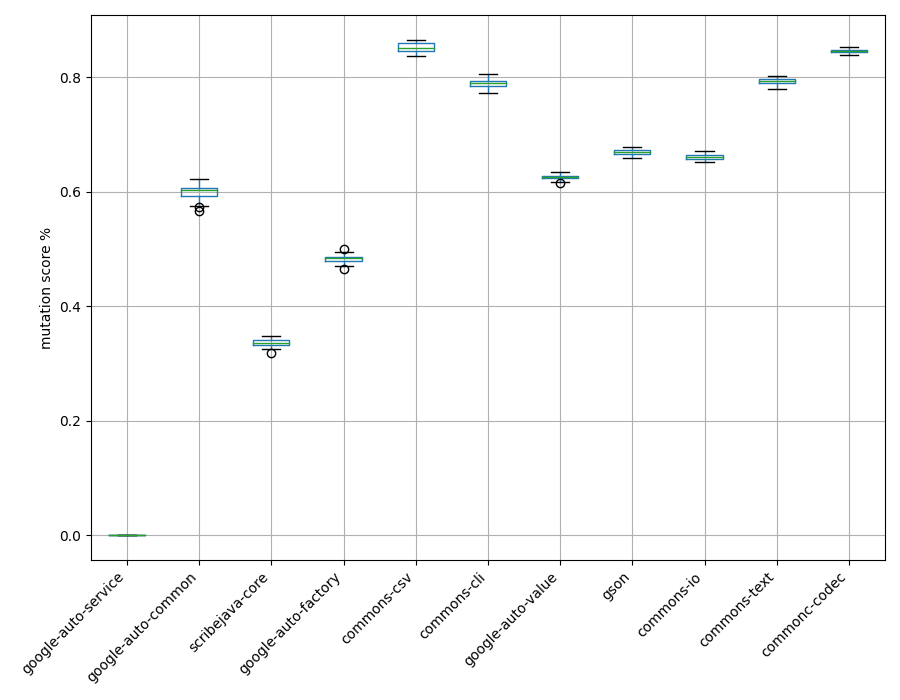
\includegraphics[width=0.5 \textwidth]{images/boxplot_summary/boxplot_hc_no_distance_0.25.png}
\caption{\label{box:clustering_no_distance_25}Box-plots containing weighted mutation score of clustering mutants without Levensthein distance and cluster size n*0.25}
\end{figure}

\begin{table*}[ht]
\centering
\begin{tabular}{|l|c|c|c|c|c|}
\hline
\multicolumn{1}{|c|}{Project} & \begin{tabular}[c]{@{}c@{}}Mutation score\\ full set\end{tabular} & \begin{tabular}[c]{@{}c@{}}Mutation score \\ clustered set\end{tabular} & \begin{tabular}[c]{@{}c@{}}Avg. cluster\\  accuracy\end{tabular} & \begin{tabular}[c]{@{}c@{}}Min. cluster\\ accuracy\end{tabular} & \begin{tabular}[c]{@{}c@{}}Max. cluster\\ accuracy\end{tabular} \\ \hline
Google Auto Service           & 0.00\%                                                                                  & 0.00\%                                                                                      & 0.00\%                                                                               & 0.00\%                                                                                & 0.00\%                                                                               \\ \hline
ScribeJava-Core               & 33.52\%                                                                                 & 33.72\%                                                                                     & 92.24\%                                                                              & 50.00\%                                                                               & 100.00\%                                                                             \\ \hline
Google Auto Factory           & 48.41\%                                                                                 & 48.32\%                                                                                     & 94.21\%                                                                              & 50.00\%                                                                               & 100.00\%                                                                             \\ \hline
Google Auto Common            & 59.59\%                                                                                 & 60.03\%                                                                                     & 91.19\%                                                                              & 50.00\%                                                                               & 100.00\%                                                                             \\ \hline
Google Auto Value             & 61.42\%                                                                                 & 62.58\%                                                                                     & 93.90\%                                                                              & 50.00\%                                                                               & 100.00\%                                                                             \\ \hline
Google Gson                   & 66.83\%                                                                                 & 66.89\%                                                                                     & 91.75\%                                                                              & 50.00\%                                                                               & 100.00\%                                                                             \\ \hline
commons-io                    & 69.70\%                                                                                 & 66.08\%                                                                                     & 90.20\%                                                                              & 50.00\%                                                                               & 100.00\%                                                                             \\ \hline
commons-cli                   & 79.07\%                                                                                 & 78.97\%                                                                                     & 91.11\%                                                                              & 50.00\%                                                                               & 100.00\%                                                                             \\ \hline
commons-text                  & 79.29\%                                                                                 & 79.30\%                                                                                     & 90.95\%                                                                              & 50.00\%                                                                               & 100.00\%                                                                             \\ \hline
commons-codec                 & 84.56\%                                                                                 & 84.59\%                                                                                     & 94.56\%                                                                              & 50.00\%                                                                               & 100.00\%                                                                             \\ \hline
commons-csv                   & 85.16\%                                                                                 & 85.24\%                                                                                     & 92.76\%                                                                              & 50.00\%                                                                               & 100.00\%                                                                             \\ \hline
\end{tabular}
\caption{\label{tab:clustering_no_distance_25}Results of clustering mutants without Levensthein distance and cluster size n*0.25}
\end{table*}

Figure \ref{box:clustering_no_distance_25} displays the box-plots of the weighted mutation score obtained from each individual sample.
We can observe that for every box-plot the \textit{p-value} is below 0.05 or 5\%.
Table \ref{tab:clustering_no_distance_25} displays the results of clustering mutants without Levensthein distance and the number of clusters equal to the total amount of mutants * 0.25. 
We observe that the maximum and minimum differences in mutation score between a full set and a clustered set  3.61\% and 0.09\% respectively.
The average of the differences between full set score and clustered score is 0.53\%.

\begin{figure}[ht]
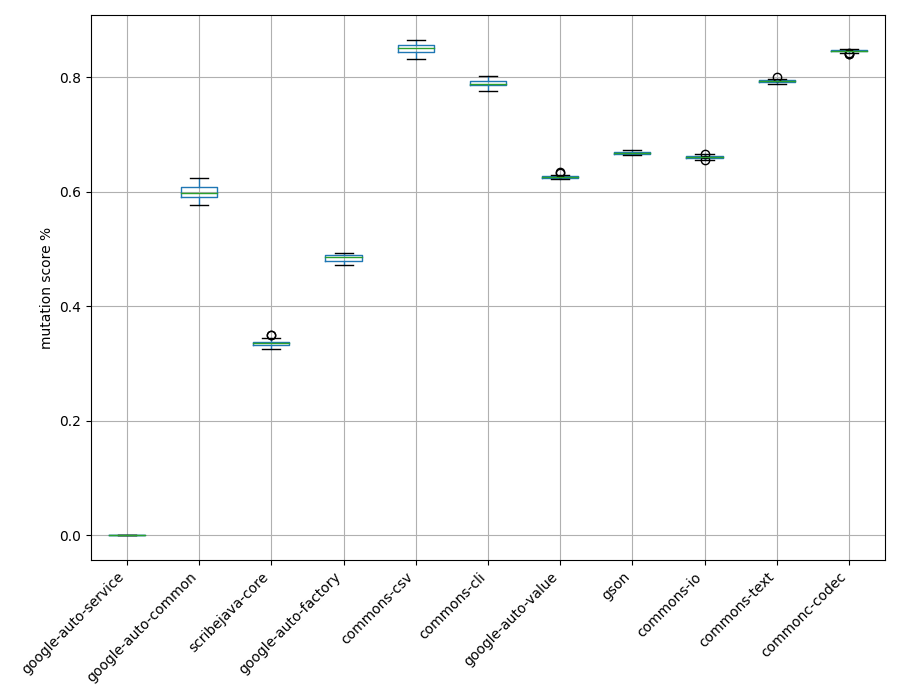
\includegraphics[width=0.5 \textwidth]{images/boxplot_summary/boxplot_hc_no_distance_0.5.png}
\caption{\label{box:clustering_no_distance_50}Box-plots containing weighted mutation score of clustering mutants without Levensthein distance and cluster size n*0.50}
\end{figure}

\begin{table*}[ht]
\centering
\begin{tabular}{|l|c|c|c|c|c|}
\hline
\multicolumn{1}{|c|}{Project} & \begin{tabular}[c]{@{}c@{}}Mutation score\\ full set\end{tabular} & \begin{tabular}[c]{@{}c@{}}Mutation score \\ clustered set\end{tabular} & \begin{tabular}[c]{@{}c@{}}Avg. cluster\\  accuracy\end{tabular} & \begin{tabular}[c]{@{}c@{}}Min. cluster\\ accuracy\end{tabular} & \begin{tabular}[c]{@{}c@{}}Max. cluster\\ accuracy\end{tabular} \\ \hline
Google Auto Service           & 0.00\%                                                                                  & 0.00\%                                                                                      & 0.00\%                                                                               & 0.00\%                                                                                & 0.00\%                                                                               \\ \hline
ScribeJava-Core               & 33.52\%                                                                                 & 33.55\%                                                                                     & 97.16\%                                                                              & 50.00\%                                                                               & 100.00\%                                                                             \\ \hline
Google Auto Factory           & 48.41\%                                                                                 & 48.44\%                                                                                     & 97.71\%                                                                              & 50.00\%                                                                               & 100.00\%                                                                             \\ \hline
Google Auto Common            & 59.59\%                                                                                 & 59.86\%                                                                                     & 96.35\%                                                                              & 50.00\%                                                                               & 100.00\%                                                                             \\ \hline
Google Auto Value             & 61.42\%                                                                                 & 62.62\%                                                                                     & 97.31\%                                                                              & 50.00\%                                                                               & 100.00\%                                                                             \\ \hline
Google Gson                   & 66.83\%                                                                                 & 66.81\%                                                                                     & 95.29\%                                                                              & 50.00\%                                                                               & 100.00\%                                                                             \\ \hline
commons-io                    & 69.70\%                                                                                 & 66.05\%                                                                                     & 95.08\%                                                                              & 50.00\%                                                                               & 100.00\%                                                                             \\ \hline
commons-cli                   & 79.07\%                                                                                 & 78.97\%                                                                                     & 95.55\%                                                                              & 50.00\%                                                                               & 100.00\%                                                                             \\ \hline
commons-text                  & 79.29\%                                                                                 & 79.30\%                                                                                     & 95.34\%                                                                              & 50.00\%                                                                               & 100.00\%                                                                             \\ \hline
commons-codec                 & 84.56\%                                                                                 & 84.59\%                                                                                     & 96.95\%                                                                              & 50.00\%                                                                               & 100.00\%                                                                             \\ \hline
commons-csv                   & 85.16\%                                                                                 & 85.11\%                                                                                     & 95.87\%                                                                              & 50.00\%                                                                               & 100.00\%                                                                             \\ \hline
\end{tabular}
\caption{\label{tab:clustering_no_distance_50}Results of clustering mutants without Levensthein distance and cluster size n*0.50}
\end{table*}

Figure \ref{box:clustering_no_distance_50} displays the box-plots of the weighted mutation score obtained from each individual sample. 
We can observe that for every box-plot the \textit{p-value} is below 0.05 or 5\%.
Table \ref{tab:clustering_no_distance_50} displays the results of clustering mutants without Levensthein distance and the number of clusters equal to the total amount of mutants * 0.50.
The maximum and minimum differences between the score of a full set and clustered set are 3.65\% and 0.03\% respectively.
We observe that the average cluster accuracy is higher than the average cluster accuracy of the 25\% set. 
The average of the differences between full set score and clustered score is 0.49\% which is smaller than the average difference than that of the 25\% set.

\begin{figure}[ht]
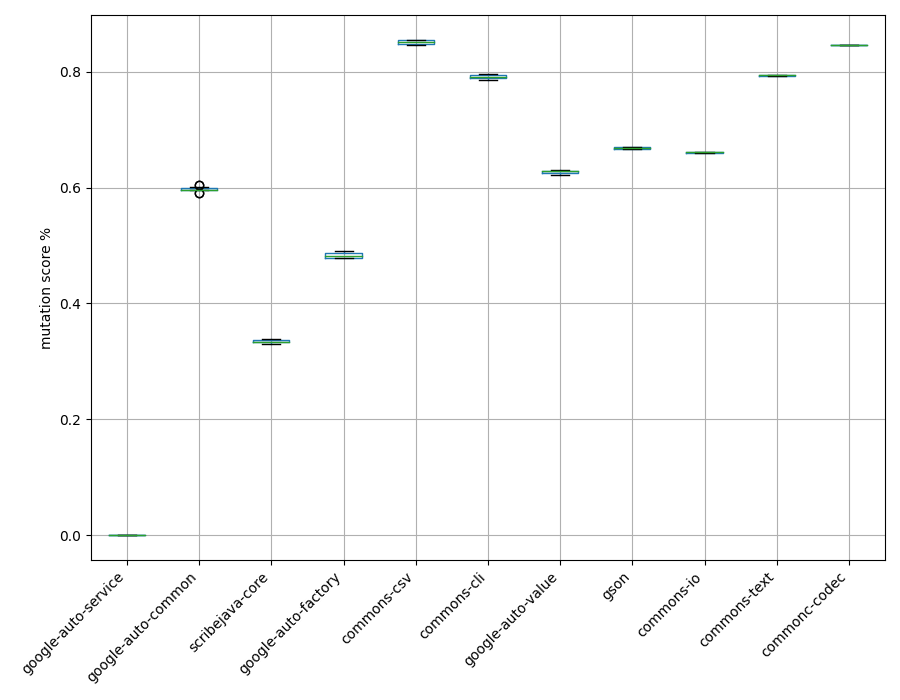
\includegraphics[width=0.5 \textwidth]{images/boxplot_summary/boxplot_hc_no_distance_0.75.png}
\caption{\label{box:clustering_no_distance_75}Box-plots containing weighted mutation score of clustering mutants without Levensthein distance and cluster size n*0.75}
\end{figure}

\begin{table*}[ht]
\centering
\begin{tabular}{|l|c|c|c|c|c|}
\hline
\multicolumn{1}{|c|}{Project} & \begin{tabular}[c]{@{}c@{}}Mutation score\\ full set\end{tabular} & \begin{tabular}[c]{@{}c@{}}Mutation score \\ clustered set\end{tabular} & \begin{tabular}[c]{@{}c@{}}Avg. cluster\\  accuracy\end{tabular} & \begin{tabular}[c]{@{}c@{}}Min. cluster\\ accuracy\end{tabular} & \begin{tabular}[c]{@{}c@{}}Max. cluster\\ accuracy\end{tabular} \\ \hline
Google Auto Service           & 0.00\%                                                                                  & 0.00\%                                                                                      & 0.00\%                                                                               & 0.00\%                                                                                & 0.00\%                                                                               \\ \hline
ScribeJava-Core               & 33.52\%                                                                                 & 33.48\%                                                                                     & 98.63\%                                                                              & 50.00\%                                                                               & 100.00\%                                                                             \\ \hline
Google Auto Factory           & 48.41\%                                                                                 & 48.34\%                                                                                     & 98.41\%                                                                              & 50.00\%                                                                               & 100.00\%                                                                             \\ \hline
Google Auto Common            & 59.59\%                                                                                 & 59.71\%                                                                                     & 97.08\%                                                                              & 50.00\%                                                                               & 100.00\%                                                                             \\ \hline
Google Auto Value             & 61.42\%                                                                                 & 62.66\%                                                                                     & 97.99\%                                                                              & 50.00\%                                                                               & 100.00\%                                                                             \\ \hline
Google Gson                   & 66.83\%                                                                                 & 66.84\%                                                                                     & 97.37\%                                                                              & 50.00\%                                                                               & 100.00\%                                                                             \\ \hline
commons-io                    & 69.70\%                                                                                 & 66.07\%                                                                                     & 97.34\%                                                                              & 50.00\%                                                                               & 100.00\%                                                                             \\ \hline
commons-cli                   & 79.07\%                                                                                 & 79.12\%                                                                                     & 96.83\%                                                                              & 50.00\%                                                                               & 100.00\%                                                                             \\ \hline
commons-text                  & 79.29\%                                                                                 & 79.33\%                                                                                     & 97.60\%                                                                              & 50.00\%                                                                               & 100.00\%                                                                             \\ \hline
commons-codec                 & 84.56\%                                                                                 & 84.61\%                                                                                     & 98.43\%                                                                              & 50.00\%                                                                               & 100.00\%                                                                             \\ \hline
commons-csv                   & 85.16\%                                                                                 & 85.07\%                                                                                     & 97.49\%                                                                              & 50.00\%                                                                               & 100.00\%                                                                             \\ \hline
\end{tabular}
\caption{\label{tab:clustering_no_distance_75}Results of clustering mutant without Levensthein distance and cluster size n*0.75}
\end{table*}

Figure \ref{box:clustering_no_distance_75} displays the box-plots of the weighted mutation score obtained from each individual sample. 
We can observe that for every box-plot the \textit{p-value} is below 0.05 or 5\%.
Table \ref{tab:clustering_no_distance_75} displays the results of clustering mutants without Levensthein distance and the number of clusters equal to the total amount of mutants * 0.50.
The maximum and minimum differences between the score of a full set and clustered set are 3.63\% and 0.04\% respectively.
We observe that the average accuracy is higher than the average accuracy of the other sets.
The average of the differences between full set score and clustered score is  0.49\% which is higher than the average difference than that of the 25\% and the same of that of the 50\% set.

\subsection{Fuzzy c-means}
\label{ch:results_rq2}
In this section we present the results of our second experiment.
We display the weighted mutation score to create box-plots.
For the same reason as in Chapter \ref{ch:results} we removed the Levenshtein distance characteristic.
\newline
The results displayed are the average of the results of the 30 repetitions of the experiment.
The result of each single repetition can be found in our Github repository in the folder \textit{experiment{\_}results}\cite{rbasarat-repo}.
Instead of displaying the reduction amount, as we did in the results of experiment one, we display the number of clusters that is calculated by the subtractive clustering model.

\begin{figure}[ht]
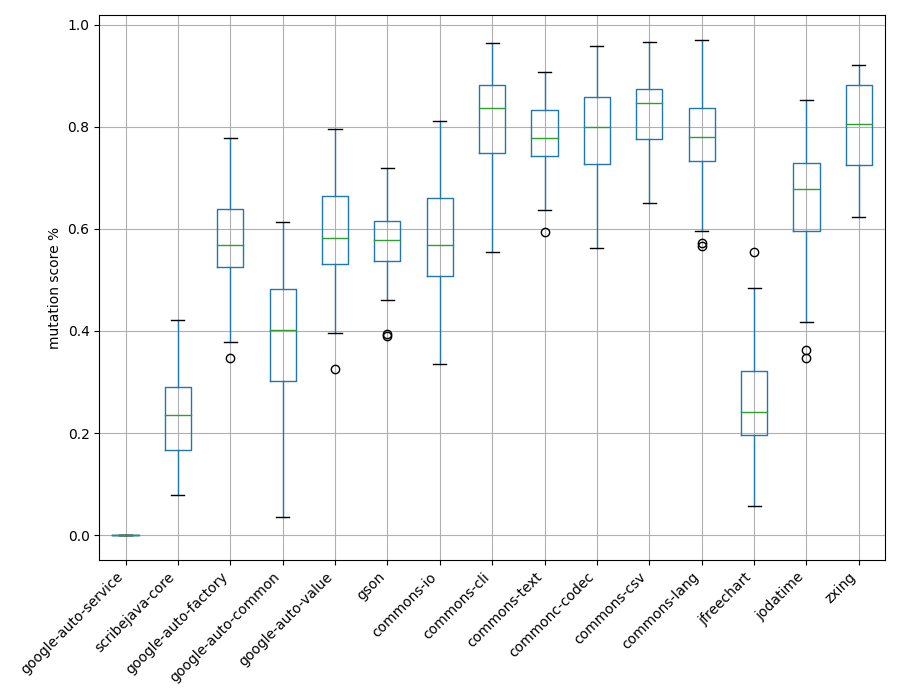
\includegraphics[width=0.5 \textwidth]{images/fcm_summary/fcm_no_distance.png}
\caption{\label{box:clustering_fcm_no_distance_25}Box-plots containing weighted mutation score of clustering mutants without Levenshtein distance characteristic.}
\end{figure}

\begin{table*}[ht]
\centering
\begin{tabular}{|l|l|l|l|l|l|l|}
\hline
Project               & \begin{tabular}[c]{@{}l@{}}Number of   \\ clusters\end{tabular} & \begin{tabular}[c]{@{}l@{}}Mutation score  \\  full set\end{tabular} & \begin{tabular}[c]{@{}l@{}}Mutation   score\\   clustered set\end{tabular} & \begin{tabular}[c]{@{}l@{}}Average cluster \\   accuracy\end{tabular} & \begin{tabular}[c]{@{}l@{}}Min. cluster   \\ accuracy\end{tabular} & \begin{tabular}[c]{@{}l@{}}Max. cluster  \\  accuracy\end{tabular} \\ \hline
Google Auto   Service & 17                   & 0.00\%                            & 0.00\%                                                 & 0.00\%                             & 0.00\%                                                                                                                                     & 0.00\%                                                                                                                                     \\ \hline
ScribeJava-Core       & 32                   & 33.52\%                           & 23.64\%                                                & 76.80\%                            & 58.77\%                                                                                                                                    & 96.60\%                                                                                                                                    \\ \hline
Google Auto   Factory & 22                   & 48.41\%                           & 57.40\%                                                & 59.20\%                            & 50.67\%                                                                                                                                    & 73.96\%                                                                                                                                    \\ \hline
Google Auto   Common  & 31                   & 59.59\%                           & 37.64\%                                                & 62.95\%                            & 50.59\%                                                                                                                                    & 83.53\%                                                                                                                                    \\ \hline
Google Auto   Value   & 41                   & 61.42\%                           & 59.61\%                                                & 61.48\%                            & 50.60\%                                                                                                                                    & 83.53\%                                                                                                                                    \\ \hline
Google Gson           & 40                   & 66.83\%                           & 57.61\%                                                & 59.11\%                            & 50.84\%                                                                                                                                    & 76.68\%                                                                                                                                    \\ \hline
Commons-io            & 40                   & 69.70\%                           & 57.95\%                                                & 57.25\%                            & 50.62\%                                                                                                                                    & 72.70\%                                                                                                                                    \\ \hline
Commons-cli           & 26                   & 79.07\%                           & 81.53\%                                                & 81.77\%                            & 67.70\%                                                                                                                                    & 95.75\%                                                                                                                                    \\ \hline
Commons-text          & 55                   & 79.29\%                           & 77.92\%                                                & 78.22\%                            & 61.80\%                                                                                                                                    & 93.92\%                                                                                                                                    \\ \hline
Commons-codec         & 17                   & 84.56\%                           & 79.46\%                                                & 77.73\%                            & 74.39\%                                                                                                                                    & 81.66\%                                                                                                                                    \\ \hline
Commons-csv           & 32                   & 85.16\%                           & 82.84\%                                                & 83.47\%                            & 65.58\%                                                                                                                                    & 97.80\%                                                                                                                                    \\ \hline
Commons-lang          & 28                   & 78.31\%                           & 76.83\%                                                & 76.99\%                            & 73.03\%                                                                                                                                    & 80.56\%                                                                                                                                    \\ \hline
Jfreechart            & 28                   & 27.02\%                           & 26.41\%                                                & 74.11\%                            & 71.83\%                                                                                                                                    & 76.36\%                                                                                                                                    \\ \hline
Jodatime              & 25                   & 70.30\%                           & 65.17\%                                                & 64.75\%                            & 60.82\%                                                                                                                                    & 69.81\%                                                                                                                                    \\ \hline
Zxing                 & 28                   & 70.64\%                           & 80.03\%                                                & 83.11\%                            & 80.10\%                                                                                                                                    & 86.03\%                                                                                                                                    \\ \hline
\end{tabular}
\caption{\label{tab:ml_no_distance}Results of clustering mutants with the fuzzy c-means model without Levenshtein distance}
\end{table*}

Figure \ref{box:clustering_fcm_no_distance_25} displays the box-plots of the weighted mutation score obtained from each individual sample. 
We can observe that for every box-plot the \textit{p-value} is more than 0.05 or 5\%.
Table \ref{tab:ml_no_distance} displays the results of clustering mutants without Levenshtein distance.
The maximum and minimum differences between the score of a full set and clustered set are 21.95\% and 0.61\% respectively.
The average of the differences between full set score and clustered score is 4.44\% which is bigger than the average difference than that of the results with all characteristics.

\section{Discussion}
The maximum deviation from the original mutation score of the experiment with hierarchical clustering, is below the statistical threshold.
We can observe that the distance between the whiskers of the box-plots do not stretch more than the \textit{alpha-value} of 0.05.
This means that there is not one sample that deviated more than 5\% from the original mutation score.
Thus we can reject the null hypothesis and accept our alternative hypothesis.
As hypothesised we observe that it is possible to cluster mutants with the set of characteristics we identified while maintaining effectiveness and reducing the amount executed.
The hypothesis holds for all the projects and variants of the experiment.
66\% of the displayed results have a deviation of less than 1\%. 
This includes both variants of the experiment.
\newline
The results prove that the relations between the mutants represented by the characteristics we identified can be used to cluster mutants efficiently. 
This can be explained by the correlation between the result of a mutant, the calculated euclidean distance and the distance threshold(linkage criteria) used to decide whether a mutants should be clustered together.
\newline
According the rules of logic, a higher cluster accuracy means a score closer to that of the original.
In other words if all clusters had an accuracy of 100\% we will achieve the same mutation score as that of the full set.
However we do not observe this behaviour in our results.
This is due to our random sampling method.
If we would select a mutant in the majority of each cluster the accuracy per cluster would correlate to the deviation in mutation score.
Unfortunately we do not know the majority of a cluster as we do now know if a mutant survives or is killed before execution.
\newline
The maximum deviation from the original mutation score of the experiment with the fuzzy c-means model, is above the statistical threshold.
We can observe that the distance between whiskers of the box-plots is more than the \textit{alpha-value} of 0.05.
Thus we cannot reject the null hypothesis and accept our alternative hypothesis.
The biggest deviation measured is 22.39\%.
This is significantly higher than the biggest deviation measured in the first experiment.
56\% of the results of both variants had a deviation in mutation score bigger than 5\%.
Our hypothesis does not hold for the clustering the mutants with the fuzzy c-means model trained in our experiment.
\newline
We observe that the number of clusters does not have an obvious relation to the total amount of mutants. 
This is expected as the subtractive clustering does not look at the total amount of data points(mutants) but to the contents(characteristics) of the data points.
The number of clusters compared to the that of the hierarchical clustering is significantly lower.
While we do not know the exact clusters centroids the subtractive model calculated, a low number of clusters indicates close relationships between certain mutants.
\newline
We observe that the minimum lowest minimum cluster accuracy measured over all variants and projects is 50.54\% with and average of 62\%. 
This is higher than the minimum of the hierarchical clustering.
This means that in all project there was not one cluster that was evenly divided.
While the minimum accuracy was higher, the maximum accuracy was lower compared to the maximum accuracy of the hierarchical clustering results.
The highest accuracy measured over all variants and projects is 97.80\% with an average of 83.79\%
This means that in all project there was not one cluster that consisted of only survived or killed mutants.
This is caused by the relatively low number of clusters.
One cluster contains more mutants which results in a bigger weight per cluster.
\section{Related work}
\label{ch:related_work}
Clustering mutants has been done before.
The research that exists tries to cluster mutants by defining the centroid of a cluster and cluster mutants on that definition.
Our research extends mutation clustering by defining a centroid that is dynamic.
In other words the centroids of our clusters are defined by the mutants itself.

\subsection{Clustering overlapped mutants}
\label{ch:overlapping_mutants}
Ma et al., clustered mutants by overlap\cite{Ma2016}.
They defined the term overlap as as mutants that are functionally equivalent.
This is close to an equivalent mutant but not the same.
They explain that an equivalent mutants is functionally identical to the original source code while an overlapped mutant is functionally identical to at least one other mutant.
If a mutant does not have an overlapped mutant that mutant would be a cluster on its own.
The achieved a reduction, in mutants executed, of 10\%.
They write in their research that it is limited to the mutator operators on expression level. 
If a mutator did not generate two or more mutants they could not detect overlapping mutants.
Their future work includes adding more mutators and widening the scope level to statements or blocks.
\newline
The research does not include efficiency.
While they show that they can cluster mutants based on overlap they do not show how efficient the mutation testing process is compared to executing a full set of mutants.
A threat to their validity, which is not addressed, is the fact that two overlapping mutants may not be challenged by the same tests and thus can result in different results.
Our research solves this problem by taking into account the location of the mutants.

\subsection{Clustering by scope}
Yu et al., extended the research about overlapping mutants(see chapter \ref{ch:overlapping_mutants})\cite{Yu2019PossibilityScope}.
They extended the scope by adding more mutators.
The also extended the research to include statements and blocks.
Their results shows an increase in clustered mutants.
The research of Yu et al., suffers from the same limitations and threats  mentioned in Chapter \ref{ch:overlapping_mutants}.

\subsection{Clustering Hamming distance}
Ji et al., did a qualitative domain analysis on mutants\cite{Ji2009}.
As a result they identified the Hamming distance to cluster with. 
The Hamming distance is, like the Levenshtein distance, a similarity measure.
They use the k-means algorithm to cluster mutants represented by Hamming distance.
They write that the reduced test set in their experiment is still as strong as the original test set\cite{Ji2009}.
\newline
Ji et al., were successful in clustering mutants with Hamming distance and the k-means algorithm.
They do acknowledge that their research still has problems with rationally determining the domains of their clusters.
Our research does not have this problem, as the centre of the domains are decided by the characteristics of the mutants.

\subsection{Spectral clustering}
Wei et al., makes use of an intelligent technique, namely spectral clustering, to improve the efficacy of mutant reduction\cite{Wei2021SpectralTesting}.
They defined multiple definitions for the mutants; similarity distance, distance between the mutants and a killing matrix of the mutants.
With these definitions they reduced the mutants based on their proposed reduction method.
This method is based on spectral clustering (SCMT), the determination method of the number of clusters, spectral clustering of mutants, and selection of representative mutants.
The reduced mutants were then clustered with a classical clustering algorithm.
Their results are promising and show high cluster accuracy.
They write that there is still work left to do in optimizing the matrices and clustering algorithms.
Our goal overlaps with that of Wei, the difference is that we used a different methodology to achieve that goal.
Another difference is that our research does not require to know the result of a mutant(killed or survived).

\subsection{Clustering similarity}
Hussain et al., used the k-means and agglomerative clustering algorithm to cluster mutants according to a similarity measure. 
They used the Hamming distance as similarity measure.
They calculated the distance and used this as data to feed into the clustering algorithms.
The number of clusters and the initial position of the cluster center in the k-means algorithm are difficult to determine, and the process of the agglomerative clustering algorithm makes it difficult to correct the existing cluster formation\cite{Hussain2008}.
They did take into account efficiency.
Hussain et al, had the same goals as our research. 
The difference is that our research used different and more elaborated methods to cluster mutants.
Hussain et al., calculated the mutation score by counting one cluster as one mutant.
Our research calculated a weighted mutation score to reflect the clusters more accurately.

\subsection{Generalizing mutants}
Wilinski et al., tried to generalize the mutants by defining metrics.
Each metric is calculated for a specific mutator.
The three metrics are usefulness, frequency and dependency.
Combining the results of usefulness and frequency metrics, they observed that reducing the number of generated mutants gives noticeable cost reduction without a loss of the mutation score accuracy.
Wilinski et al., their research is narrowly scoped to the specific mutators they decided to do research on.
Our research does not contain this limitation.
The mutator is used as a characteristic in our research instead of limiting our research it helps define a mutant.

\section{Conclusion}
\label{ch:conclusion}
Our research started with comparing three mutation testing tools for Java and found that the state of the art was outdated.
We replicated that research with data currently available on the mutation testing tools.
This new information showed that two out of three mutation testing tools were not actively maintained anymore.
The mutation testing tool PIT scored best on the metrics measured in our replication study, this is also the tool we decided to use for our research.
\newline
We performed a qualitative analysis on mutant characteristics.
As a result we created a list of identified characteristics based on existing research. 
We then extended this list by identifying characteristic with logic and data available.
We used the identified characteristics to represent the mutants.
\newline
We clustered the mutants with a white box approach and a black box approach.
For our white box approach we selected the hierarchical clustering algorithm.
The hierarchical clustering showed that we can cluster mutants while maintaining effectiveness.
We achieved reductions of up to 75\% of the total amount of mutants without significantly reducing the accuracy.
\newline
For the black box approach we selected a machine learning model, specifically the fuzzy c-means model.
The fuzzy c-means model showed a significant reduction in effectiveness.
We trained the fuzzy c-means model with parameters that were optimal according to existing research. 
We used a different machine learning model, specialized in calculating the number of clusters for fuzzy clustering, to calculate the number of clusters.
While the minimum clustering accuracy was higher than that of the hierarchical clustering, the maximum cluster accuracy was lower than that of the hierarchical clustering.
The cluster accuracy had a larger impact on the clusters of the machine learning model because there was a relatively small number of clusters.
Our research proves that it is possible to determine the means of domains as the centre of a cluster within a programming language without narrowing down the scope to specific pieces of code.
The centroids our research identified is decided by the characteristics of the mutants.
It can be applied to all Java projects that can be run with PIT. 
Which is a larger scope than in existing mutation clustering research.

\printbibliography[heading=bibintoc]

\end{document}
